\documentclass[12pt]{article}

\usepackage[a4paper, margin=1in]{geometry}
\usepackage[english]{babel}
\usepackage[utf8]{inputenc}

\usepackage[colorlinks=true, allcolors=blue]{hyperref}

\title{CRPL: Interim Report}
\author{Harrison Beau Barker}

\usepackage{graphicx}
\graphicspath{ {images/} }

\usepackage{xcolor}

\usepackage{tabularx}
\newcolumntype{b}{X}
\newcolumntype{s}{>{\hsize=.5\hsize}X}

\newcommand{\keyword}[1]{\textbf{\textit{#1}}}
\newcommand{\q}[2]{\begin{quote} #1 \cite{#2} \end{quote}}

\setlength{\parskip}{1em}
%\setlength{\parindent}{0em}
\begin{document}

\begin{titlepage}
	\centering
	
\includegraphics[width=0.4\textwidth]{crpl}\par
	\vspace{1cm}
	{\huge\bfseries CRPL: Report\par}
	\vspace{2cm}
	{\Large\itshape Harrison Beau Barker\par}
	\vfill
	{\url{https://github.com/MrHarrisonBarker/crpl}\par}
	\vspace{1cm}
	{\large Hbark002, 33575210\par}
\end{titlepage}

\abstract{TODO}

\tableofcontents{}

\section{Keywords}

\section{Introduction}
% TODO The problem. Take inspiration from the presentation

The aim of this project is to represent a version of \keyword{copyright} for protection of intellectual property on a \keyword{blockchain} backed by a public ledger of transactions. My initial impetus for this project was a book I read in 2018 called \textit{"Blockchain Revolution: How the Technology Behind Bitcoin Is Changing Money, Business, and the World"}\cite{blockchain_revolution}, before this point I knew little of the applications for blockchain technologies attributing them only to a new form of digital currency allowing peer to peer transactions of wealth.

However, this book introduced the concept of \keyword{smart contracts} and the possibilities now small immutable programs could be saved and run on a blockchain. The most relevant change smart contracts brought was progressive state into an infamously immutable technology, by leveraging an unmodifiable chain of transactions state became not just a current record (like most traditional systems) but a historical account of all previous states with a clear a definable list of transformations precisely timestamped.

This new knowledge of \keyword{blockchains} came to fruition when it came to selecting my final project but to what problem should I help to provide a solution to leveraging this technology. A combination of recent interest in the crypto-sphere mainly coming from NFTs, continued displays of a \keyword{copyright} system not fit for purpose\cite{DMCA-abuse} and the book I had read 3 years earlier proposing that \keyword{blockchain} and \keyword{smart contracts} were an extremely viable solution to problems intersecting law and social structures.

\subsection{Unfit for purpose}

% general complexity
% complexity from different countries laws
% digital world is global so should copyright
% computerised and open

Focusing on the problem at hand being the current copyright system is not fit for its purpose. 

\subsection{What a solution needs}

% TODO what is needed of a solution to fix this problem?

\section{Research}
\subsection{Blockchain}
% TODO Technical knowledge needed to implement
% TODO How it works?
% TODO Why use it?

\subsection{Existing solutions}

\subsubsection{Copyright law}
% TODO The state of the current copyright system
\subsubsection{Online rights management}
% TODO How do creators manage protection of their work

\subsection{Development theory}
% TODO Explanation of agile development methodology
% TODO TDD and Scrum

\subsection{Aims of the solution}
% TODO The over arcing aims of the solution, aka what should the system fix

\section{Design}

\subsection{Technical Requirements}
% TODO a more comprehensive and detailed list of requirements

\begin{description}
	\item[Copyright smart contract] Immutable code on a public ledger “blockchain“ for the purpose of establishing ownership or the copyright to a piece of work.
	\item[Multi-party distribution] The ability to establish a complex ownership structure which includes multiple individuals/groups.
	\item[Ownership transfer] The ability to change the ownership of a copyright from one complex structure to another with consent of all current owner(s).
	\item[Work verification] Verification of a work to establish its originality with a reasonable accuracy for the platform.
	\item[Dispute filing] Allow any user to dispute a copyright with sufficient evidence and provide an option for resolving these disputes by the owner(s).
	\item[Digital signing] Digital signing a work for authentic verification based on our records.
	\item[\color{orange}{Decentralised Work CDN & proxy}] Providing an access point for stored work within the chain.
	\item[\color{orange}{Web-socket updates}] Real-time updates for the front-end UI to provide a better end-user experience.
\end{description}

\subsection{Smart contract}
% TODO Ownership structure
% TODO Permission based protections
% TODO Inspiration from nft contract (starting point) https://eips.ethereum.org/EIPS/eip-721
% TODO Shareholder consensus mechanism

\subsection{Back-end}
% TODO Service and dependancy injection based architecture
% TODO Background service pattern
% TODO event processing patterns
% TODO state diagrams (how the flow of applications)

\subsection{Database}
% TODO what is duplicated between the chain and the database
% TODO what is only on the database and not on the chain
% TODO Express the need for synchronisation

\subsection{Front-end}
% TODO Visual design philosophy
% TODO How the use will login?
% TODO form design and working

\subsection{Development process}
% TODO how the development was laid out and planned
% TODO sprint structure

\section{Implementation}

\subsection{Smart contract}
% TODO saved metadata

\subsubsection{Interface overview}
% TODO events
% TODO ownership
% TODO copyright

\subsubsection{Registration}
% TODO Registration of copyright
% TODO how each copyright is saved (maximum size?)
% TODO approve the message sender
% TODO record all shareholders

\subsubsection{Ownership restructure}
% TODO Restructure proposal
% TODO Binding vote
% TODO Restructure event
% TODO failed restructure

\subsubsection{Modifiers}
% TODO isShareholder or approved
% TODO valid addresses
% TODO expired

\subsection{Back-end}
% TODO Service -> Controller
% TODO digital signing
% TODO ContractRepository

\subsubsection{Queries}
% TODO structured query
% TODO chain injection
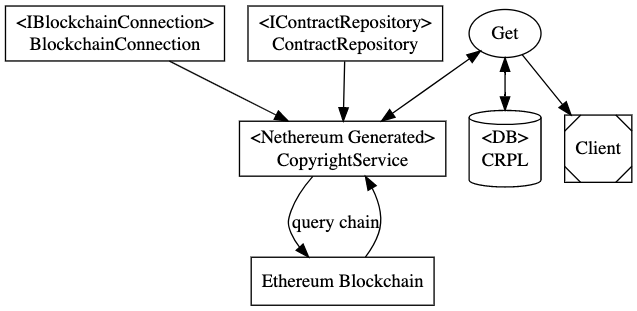
\includegraphics[width=\textwidth,height=\textheight,keepaspectratio]{images/operational/chain-inject}

\subsubsection{Registration process}
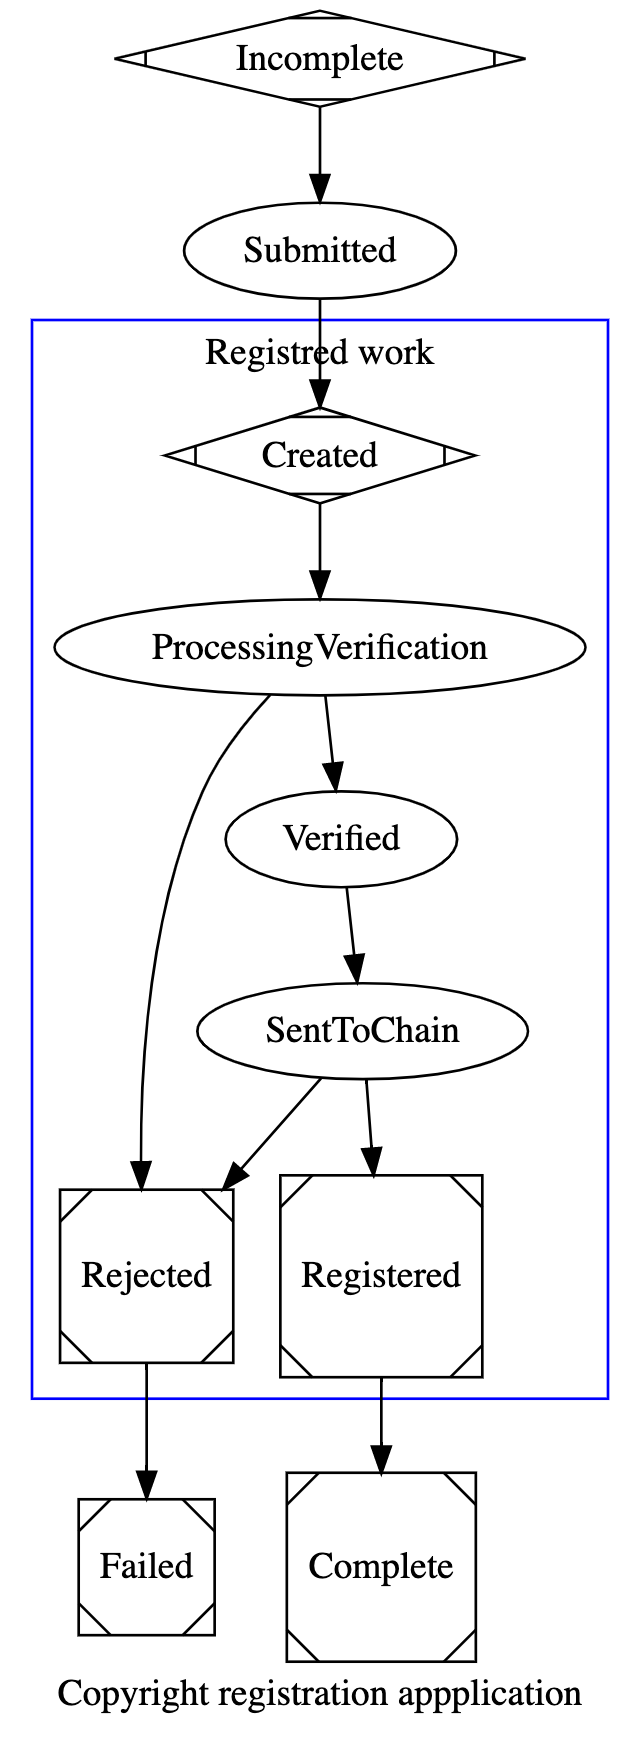
\includegraphics[width=\textwidth,height=\textheight,keepaspectratio]{images/operational/cpy-registration-status-graph}

\subsubsection{Dispute handling}
% TODO filing disputes
% TODO resolving disputes: payment, change of ownership
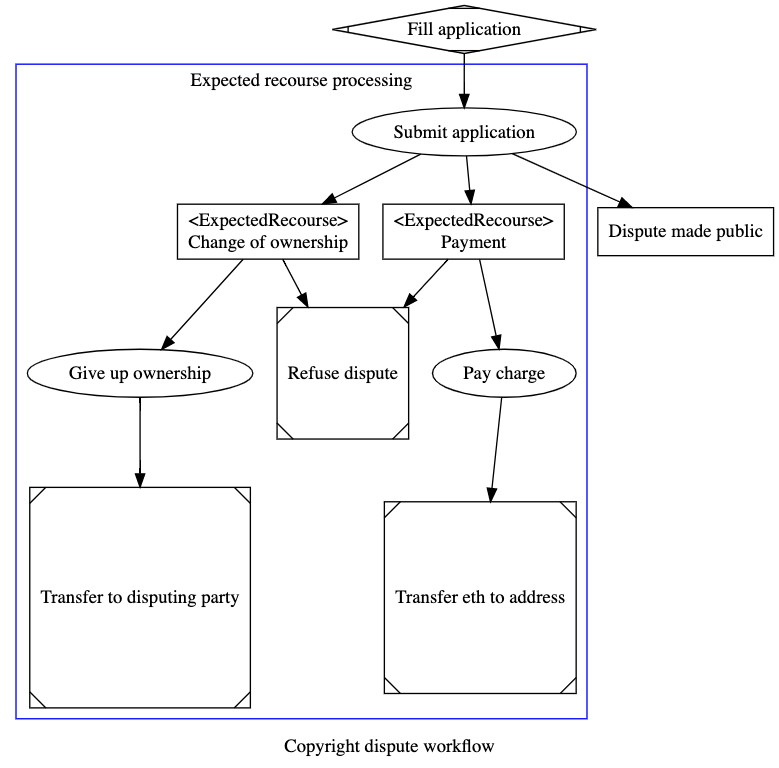
\includegraphics[width=\textwidth,height=\textheight,keepaspectratio]{images/operational/dispute-workflow}

\subsubsection{Applications framework}
% TODO Data model structure (application, view model, input model)
% TODO unified status and processing flow (update -> submit = complete)

\subsubsection{API overview}
% TODO API diagrams and structure
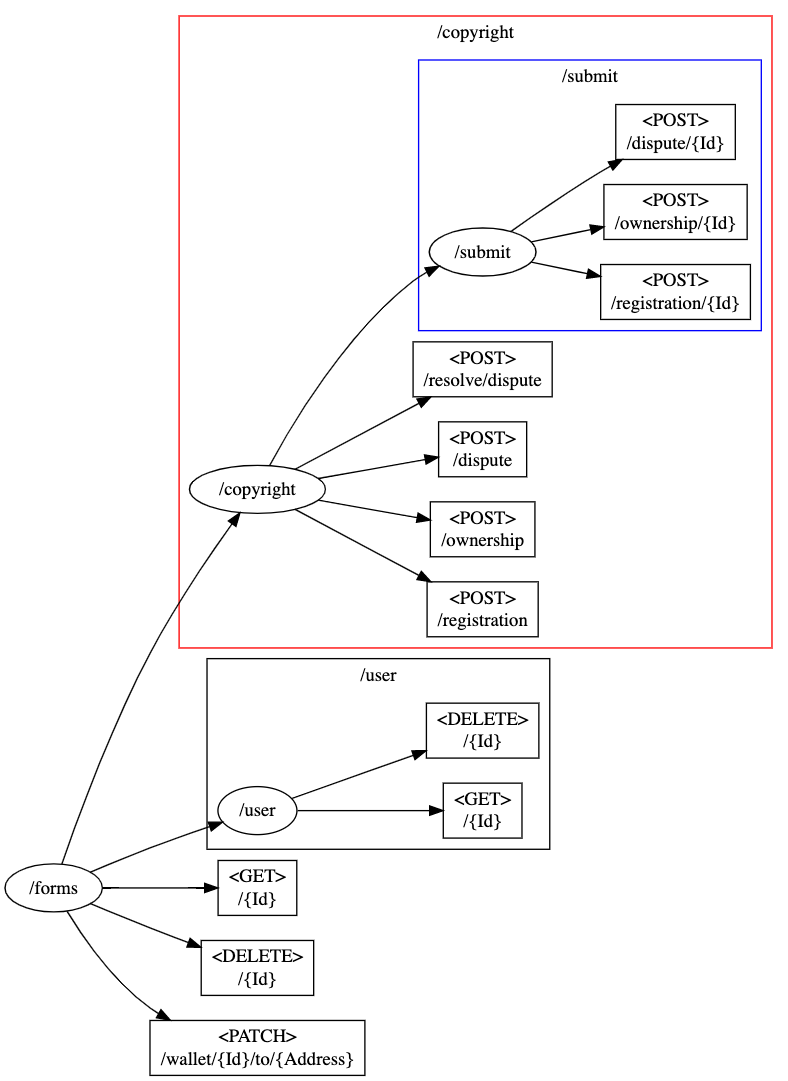
\includegraphics[width=\textwidth,height=\textheight,keepaspectratio]{images/operational/Forms-Api}

\subsubsection{Blockchain event listeners}
% TODO Blockchain event listeners
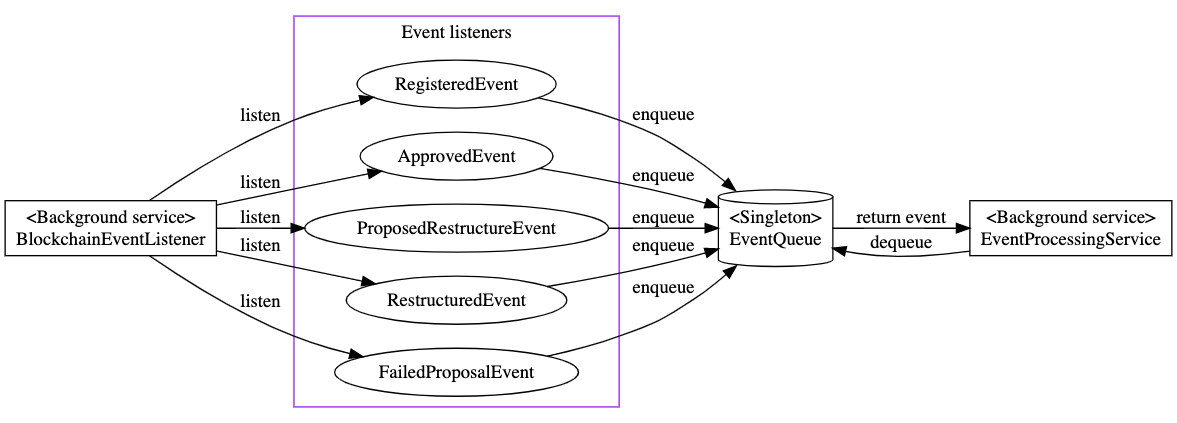
\includegraphics[width=\textwidth,height=\textheight,keepaspectratio]{images/operational/Event-Listening}


\subsubsection{Background services}
% TODO verification pipeline
% TODO Expiry

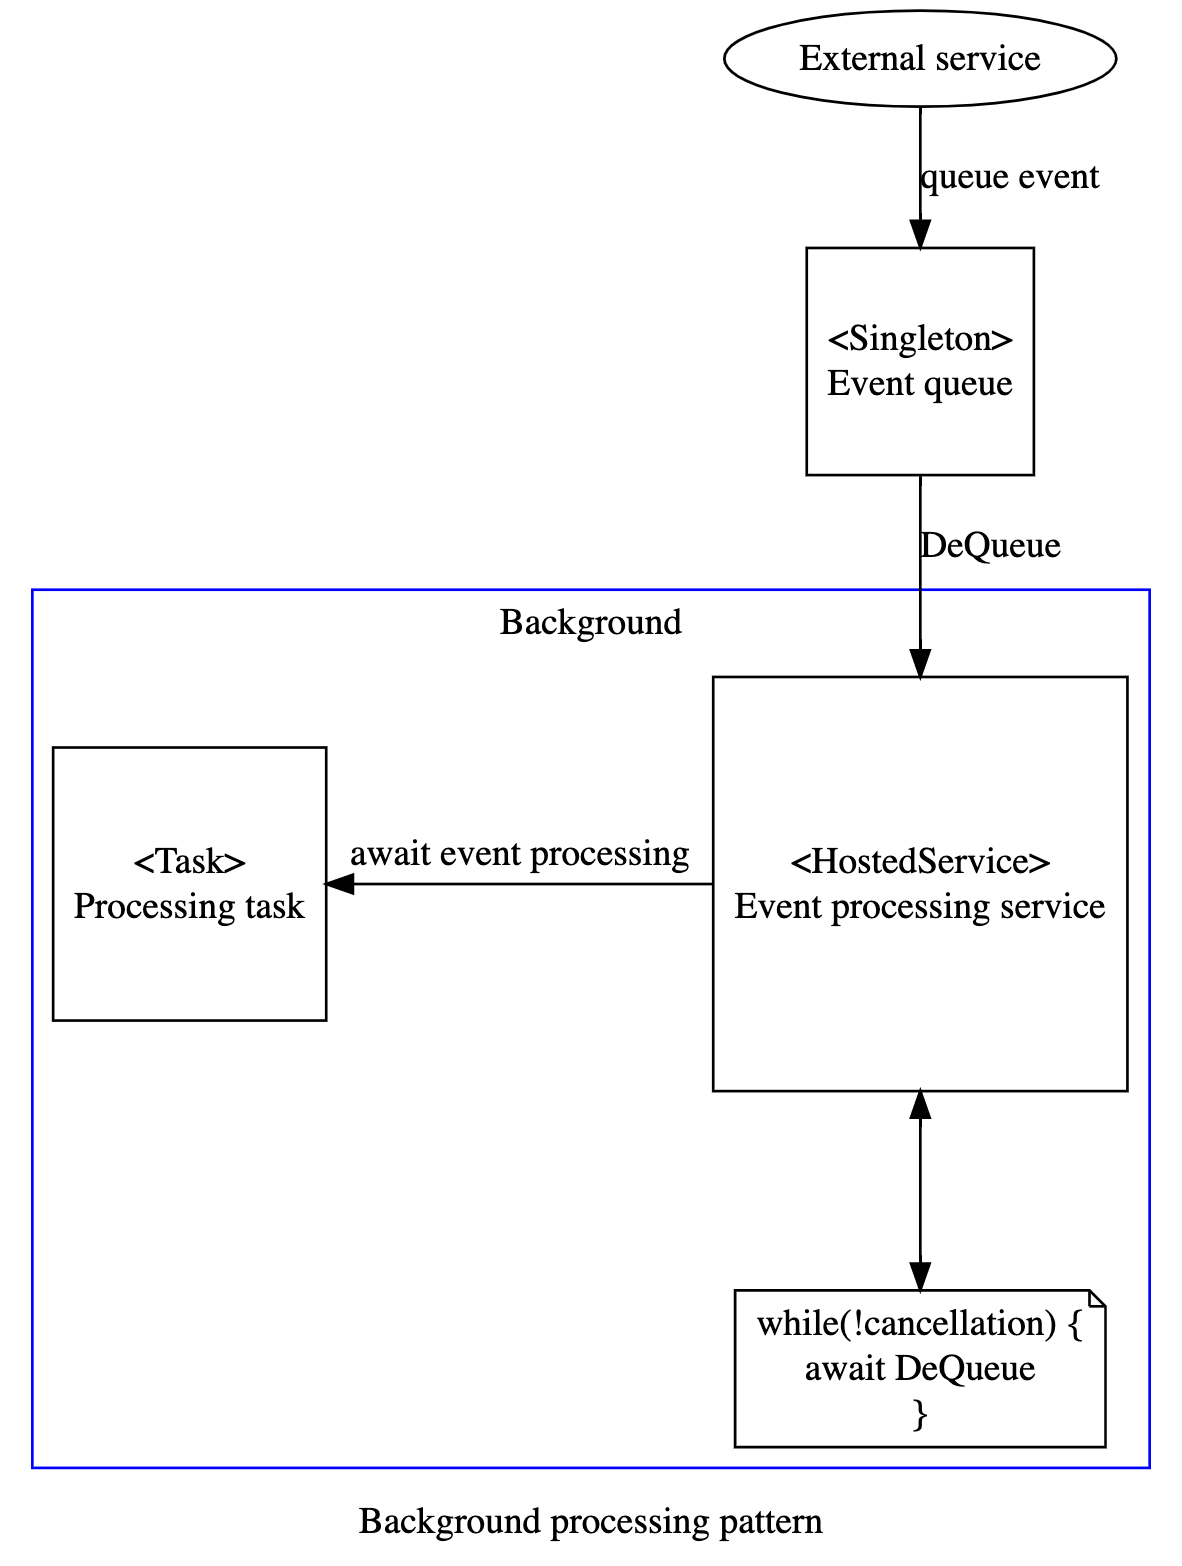
\includegraphics[width=\textwidth,height=\textheight,keepaspectratio]{images/patterns/background-processing-pattern}

\subsubsection{Account management}
% TODO issues with transfer and delete account

\subsection{Database}
% TODO ChainSync™

\subsection{Front-end}

\section{Discussion}
\subsection{Limitation}
% TODO limits of the scope (having to reign in the scope of the project at all points)
% TODO limits of the implementation (gas/price aka no money involved at the moment, transfer and delete wallet, de-sync)

\subsection{Blockchain technology}
% TODO Are these NFTs?
% TODO How long will the blockchain?
% TODO Social consensus/ conflict with governments

\section{Evaluation}
\subsection{Process}
% TODO evaluating my development
% TODO was development agile?

\subsection{Product}
% TODO Has all the functional specifications been met
% TODO Has all the non-functional specs been met
% TODO Does the product fit the target users needs
% TODO Does the product fulfil

\section{Future development}

\begin{description}
	\item[Royalty payments]
	\item[External verification]
	\item[Analytics]
\end{description}

\section{Conclusion}


\bibliographystyle{plain}
\bibliography{sources.bib}

\end{document}
